% !TEX spellcheck = en_US



% ~~~~~~~~~~~~~~~~~~~~~~~~~~~~~~~~~~~~~~~ V
% (NC) 2026 Haluk Bingol
% github.com/halukbingol/LaTeX-Templates
%
% Licensees may copy, distribute, display, and perform the work and make derivative works 
% and remixes based on it only for non-commercial purposes. 
% ~~~~~~~~~~~~~~~~~~~~~~~~~~~~~~~~~~~~~~~ A




% =====================================================================
%  Regular Expressions in Java -- Sophomore Level: Pattern, Matcher, Groups and Flags
%  ---------------------------------------------------------------------
%  Built on hblib/Template/hblibTemplate.tex with the libraries in ../../hblib/.
%  Programs and their real outputs are in codeoutput/:
%     codeoutput/<Name>.java  a program (classes without main() are only compiled)
%     codeoutput/<Name>.sh    a terminal session, run in a copy of codeoutput/<Name>/
%     codeoutput/<Name>.txt   what it printed, made by:  bash run_examples.sh
% =====================================================================

\documentclass[aspectratio=169,10pt,compress]{beamer}

% ~~~~~~~~~~~~~~~~~~~~~~~~~~~~~~~~~~~~~~~~~~~~~~~~~~~~~~~~~~~~~~~~~ V hblib
	\usepackage{../../hblib/hblibPresentation} % lib presentation: theme, i/N, \hSection, algorithm2e, ...
	\usepackage{../../hblib/hblibCodeoutput} % lib code + output: \lstcode, \lstterminal, ...
	\usepackage{../../hblib/hblibDatastructures} % lib data structures: \hString, \hStack, \hQueue
% ~~~~~~~~~~~~~~~~~~~~~~~~~~~~~~~~~~~~~~~~~~~~~~~~~~~~~~~~~~~~~~~~~ A hblib


% theme, i/N, fonts (T1, lmodern), booktabs, xcolor, array (L{width} columns), listings, tikz,
% algorithm2e (\small captions, \Fn) and the color gitred come from the hblib libraries




% +++++++++++++++++++++++++++++++++++++++ V specific
\DontPrintSemicolon % in algorithms
\newcommand{\win}{\textbf{Windows}}
\newcommand{\mac}{\textbf{macOS}}
% +++++++++++++++++++++++++++++++++++++++ A specific

% ---------------------------------------------------------------------
\title{Regular Expressions in Java}
\subtitle{Sophomore Level: Pattern, Matcher, Groups and Flags}
\author[Bingol]{Haluk O. Bingol}

\institute[FCIS]{
    Faculty of Computer and Information Sciences\\
    Yeditepe University
}
\date{
	{\tiny \hbTimeStamp}
}

\begin{document}




% ~~~~~~~~~~~~~~~~~~~~~~~~~~~~~~~~~~~~~~ V frm
\begin{frame}[t,fragile]
  \titlepage
\end{frame}
% ~~~~~~~~~~~~~~~~~~~~~~~~~~~~~~~~~~~~~~ A frm




% ~~~~~~~~~~~~~~~~~~~~~~~~~~~~~~~~~~~~~~ V frm
\begin{frame}[t,fragile] \frametitle{Outline}
  \begin{columns}[T]
    \begin{column}{0.48\textwidth}
      \tableofcontents[sections={1-4}, hideallsubsections]
    \end{column}
    \begin{column}{0.48\textwidth}
      \tableofcontents[sections={5-8}, hideallsubsections]
    \end{column}
  \end{columns}
\end{frame}
% ~~~~~~~~~~~~~~~~~~~~~~~~~~~~~~~~~~~~~~ A frm

% ~~~~~~~~~~~~~~~~~~~~~~~~~~~~~~~~~~~~~~ V
\hSection[API]{Pattern and Matcher}
% ~~~~~~~~~~~~~~~~~~~~~~~~~~~~~~~~~~~~~~ A




% ~~~~~~~~~~~~~~~~~~~~~~~~~~~~~~~~~~~~~~ V frm
\begin{frame}[t,fragile] \frametitle{Two classes in \texttt{java.util.regex}}
  \begin{columns}[T]
    \begin{column}{0.5\textwidth}
      \begin{center}
      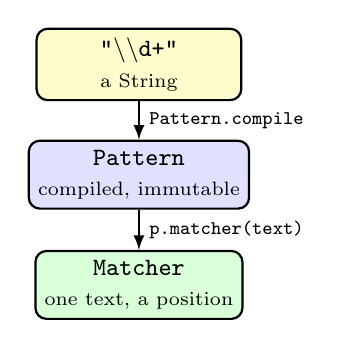
\begin{tikzpicture}[b/.style={draw, thick, rounded corners, minimum width=2.6cm, minimum height=0.8cm, font=\small, align=center}]
        \node[b, fill=yellow!20] (s) at (0,2.4)  {\texttt{"\textbackslash\textbackslash d+"}\\ \scriptsize a String};
        \node[b, fill=blue!12]   (p) at (0,1.0)  {\texttt{Pattern}\\ \scriptsize compiled, immutable};
        \node[b, fill=green!15]  (m) at (0,-0.4) {\texttt{Matcher}\\ \scriptsize one text, a position};
        \draw[-latex, thick] (s) -- node[right, font=\scriptsize] {\texttt{Pattern.compile}} (p);
        \draw[-latex, thick] (p) -- node[right, font=\scriptsize] {\texttt{p.matcher(text)}} (m);
      \end{tikzpicture}
      \end{center}
    \end{column}
    \begin{column}{0.46\textwidth}
      \begin{itemize}\small
        \item \texttt{Pattern}: compile once (\texttt{static final}), use many times, safe to share between threads.
        \item \texttt{Matcher}: walks over one text; keeps where the last match was. Not thread-safe.
        \item \texttt{String.matches}, \texttt{split}, \texttt{replaceAll} compile the pattern \textbf{every time}.
      \end{itemize}
      \begin{center}\footnotesize
      \begin{tabular}{@{}ll@{}}
        \toprule
        \texttt{m.matches()}   & the whole text \\
        \texttt{m.lookingAt()} & from the start \\
        \texttt{m.find()}      & the next match anywhere \\
        \bottomrule
      \end{tabular}
      \end{center}
    \end{column}
  \end{columns}
\end{frame}
% ~~~~~~~~~~~~~~~~~~~~~~~~~~~~~~~~~~~~~~ A frm




% ~~~~~~~~~~~~~~~~~~~~~~~~~~~~~~~~~~~~~~ V frm
\begin{frame}[t,fragile] \frametitle{\texttt{find} in a loop}
  \lstcoderightstep[0.62][basicstyle=\ttfamily\tiny][basicstyle=\ttfamily\scriptsize]{codeoutput/Find.java}{Java}{codeoutput/Find.txt}

  \vspace{0.2em}
  \small \texttt{group()} is the whole match, \texttt{group(1)}, \texttt{group(2)} the parts in parentheses; \texttt{start}/\texttt{end}: positions (end exclusive). \texttt{cis111} matches too: \texttt{[A-Za-z]}.
\end{frame}
% ~~~~~~~~~~~~~~~~~~~~~~~~~~~~~~~~~~~~~~ A frm

% ~~~~~~~~~~~~~~~~~~~~~~~~~~~~~~~~~~~~~~ V
\hSection[Groups]{Groups}
% ~~~~~~~~~~~~~~~~~~~~~~~~~~~~~~~~~~~~~~ A




% ~~~~~~~~~~~~~~~~~~~~~~~~~~~~~~~~~~~~~~ V frm
\begin{frame}[t,fragile] \frametitle{Named groups: \texttt{(?<name>\dots)}}
  \lstcoderightstep[0.62][basicstyle=\ttfamily\tiny][basicstyle=\ttfamily\scriptsize]{codeoutput/Named.java}{Java}{codeoutput/Named.txt}

  \vspace{0.2em}
  \small A name says more than a number, and survives when the pattern changes. In a replacement: \texttt{\$\{name\}}.
\end{frame}
% ~~~~~~~~~~~~~~~~~~~~~~~~~~~~~~~~~~~~~~ A frm

% ~~~~~~~~~~~~~~~~~~~~~~~~~~~~~~~~~~~~~~ V
\hSection[Flags]{Flags}
% ~~~~~~~~~~~~~~~~~~~~~~~~~~~~~~~~~~~~~~ A




% ~~~~~~~~~~~~~~~~~~~~~~~~~~~~~~~~~~~~~~ V frm
\begin{frame}[t,fragile] \frametitle{Case, comments, lines, dot}
  \lstcoderightstep[0.62][basicstyle=\ttfamily\tiny][basicstyle=\ttfamily\scriptsize]{codeoutput/Flags.java}{Java}{codeoutput/Flags.txt}

  \vspace{0.2em}
  \small \texttt{COMMENTS}: spaces ignored, \texttt{\#} starts a comment.
  \texttt{MULTILINE}: \texttt{\textasciicircum} and \texttt{\$} at every line. \texttt{(?s)} = \texttt{DOTALL}: \texttt{.} matches a newline, too.
\end{frame}
% ~~~~~~~~~~~~~~~~~~~~~~~~~~~~~~~~~~~~~~ A frm

% ~~~~~~~~~~~~~~~~~~~~~~~~~~~~~~~~~~~~~~ V
\hSection[Parsing]{Parsing Text}
% ~~~~~~~~~~~~~~~~~~~~~~~~~~~~~~~~~~~~~~ A




% ~~~~~~~~~~~~~~~~~~~~~~~~~~~~~~~~~~~~~~ V frm
\begin{frame}[t,fragile] \frametitle{Reading a log file}
  \begin{columns}[T]
    \begin{column}{0.49\textwidth}
      \lstcode[basicstyle=\ttfamily\tiny, lastline=14]{codeoutput/Logs.java}{Java}
    \end{column}
    \begin{column}{0.49\textwidth}
      \lstcode[basicstyle=\ttfamily\tiny, firstline=15, firstnumber=15]{codeoutput/Logs.java}{Java}
    \end{column}
  \end{columns}
\end{frame}
% ~~~~~~~~~~~~~~~~~~~~~~~~~~~~~~~~~~~~~~ A frm




% ~~~~~~~~~~~~~~~~~~~~~~~~~~~~~~~~~~~~~~ V frm
\begin{frame}[t,fragile] \frametitle{The errors and the count}
  \begin{columns}[T]
    \begin{column}{0.5\textwidth}
      \lstoutput[basicstyle=\ttfamily\scriptsize]{codeoutput/Logs.txt}
    \end{column}
    \begin{column}{0.46\textwidth}
      \begin{itemize}\small
        \item One pattern describes a whole line: date, time, level, message.
        \item \texttt{MULTILINE} + \texttt{\textasciicircum}\dots\texttt{\$}: every line separately; ``garbage line'' is skipped.
        \item \texttt{(INFO|WARN|ERROR)}: \textbf{alternation}, one of three.
      \end{itemize}
    \end{column}
  \end{columns}
\end{frame}
% ~~~~~~~~~~~~~~~~~~~~~~~~~~~~~~~~~~~~~~ A frm




% ~~~~~~~~~~~~~~~~~~~~~~~~~~~~~~~~~~~~~~ V frm
\begin{frame}[t,fragile] \frametitle{Replacing with a function}
  \lstcoderightstep[0.62][basicstyle=\ttfamily\tiny][basicstyle=\ttfamily\scriptsize]{codeoutput/ReplaceFn.java}{Java}{codeoutput/ReplaceFn.txt}

  \vspace{0.2em}
  \small \texttt{Matcher.replaceAll(m -> \dots)} (Java 9+) computes each replacement from the match: here +20\,\% prices and capital initials.
  \texttt{\textbackslash p\{L\}}: any letter, also \texttt{ş}, \texttt{ı}.
\end{frame}
% ~~~~~~~~~~~~~~~~~~~~~~~~~~~~~~~~~~~~~~ A frm

% ~~~~~~~~~~~~~~~~~~~~~~~~~~~~~~~~~~~~~~ V
\hSection[Look-ahead]{Look-ahead: Several Rules at Once}
% ~~~~~~~~~~~~~~~~~~~~~~~~~~~~~~~~~~~~~~ A




% ~~~~~~~~~~~~~~~~~~~~~~~~~~~~~~~~~~~~~~ V frm
\begin{frame}[t,fragile] \frametitle{A password policy}
  \lstcoderightstep[0.5][basicstyle=\ttfamily\tiny][basicstyle=\ttfamily\tiny]{codeoutput/Password.java}{Java}{codeoutput/Password.txt}

  \vspace{0.2em}
  \small \texttt{(?=.*\textbackslash d)} checks ``a digit follows somewhere'' without consuming characters; four look-aheads, then \texttt{.\{8,\}} for the length.
  Separate checks give the user a better message than one big pattern.
\end{frame}
% ~~~~~~~~~~~~~~~~~~~~~~~~~~~~~~~~~~~~~~ A frm

% ~~~~~~~~~~~~~~~~~~~~~~~~~~~~~~~~~~~~~~ V
\hSection[Greedy]{Greedy and Lazy}
% ~~~~~~~~~~~~~~~~~~~~~~~~~~~~~~~~~~~~~~ A




% ~~~~~~~~~~~~~~~~~~~~~~~~~~~~~~~~~~~~~~ V frm
\begin{frame}[t,fragile] \frametitle{\texttt{.*} takes as much as it can}
  \lstcoderightstep[0.56][basicstyle=\ttfamily\tiny][basicstyle=\ttfamily\tiny]{codeoutput/Greedy.java}{Java}{codeoutput/Greedy.txt}

  \vspace{0.2em}
  \small \texttt{.*} is \textbf{greedy}: up to the \emph{last} \texttt{</b>}. \texttt{.*?} is \textbf{lazy}: as little as possible. Best: say exactly what may appear, \texttt{[\textasciicircum<]*}.
\end{frame}
% ~~~~~~~~~~~~~~~~~~~~~~~~~~~~~~~~~~~~~~ A frm

% ~~~~~~~~~~~~~~~~~~~~~~~~~~~~~~~~~~~~~~ V
\hSection[Quality]{Reusing and Testing Patterns}
% ~~~~~~~~~~~~~~~~~~~~~~~~~~~~~~~~~~~~~~ A




% ~~~~~~~~~~~~~~~~~~~~~~~~~~~~~~~~~~~~~~ V frm
\begin{frame}[t,fragile] \frametitle{Compile once, use many times}
  \lstcoderightstep[0.62][basicstyle=\ttfamily\tiny][basicstyle=\ttfamily\scriptsize]{codeoutput/Reuse.java}{Java}{codeoutput/Reuse.txt}

  \vspace{0.2em}
  \small \texttt{asMatchPredicate}: the whole string must match; \texttt{asPredicate}: a match \emph{somewhere} is enough, so
  ``\texttt{to: deniz@\dots}'' counts too. \texttt{std\_yeditepe} fails: the dot is escaped (\texttt{\textbackslash\textbackslash .}).
\end{frame}
% ~~~~~~~~~~~~~~~~~~~~~~~~~~~~~~~~~~~~~~ A frm




% ~~~~~~~~~~~~~~~~~~~~~~~~~~~~~~~~~~~~~~ V frm
\begin{frame}[t,fragile] \frametitle{Test your patterns}
  \begin{columns}[T]
    \begin{column}{0.5\textwidth}
      \lstcode[basicstyle=\ttfamily\tiny]{codeoutput/Tests/CourseCode.java}{Java}
      \lstcode[basicstyle=\ttfamily\tiny, firstline=6, firstnumber=6]{codeoutput/Tests/CourseCodeTest.java}{Java}
    \end{column}
    \begin{column}{0.48\textwidth}
      \uncover<2->{\lstterminal[basicstyle=\ttfamily\tiny]{codeoutput/Tests.txt}}
      \small A regex is code: test the valid \emph{and} the invalid inputs, especially the borders (JUnit deck).
    \end{column}
  \end{columns}
\end{frame}
% ~~~~~~~~~~~~~~~~~~~~~~~~~~~~~~~~~~~~~~ A frm

% ~~~~~~~~~~~~~~~~~~~~~~~~~~~~~~~~~~~~~~ V
\hSection[Summary]{Summary}
% ~~~~~~~~~~~~~~~~~~~~~~~~~~~~~~~~~~~~~~ A




% ~~~~~~~~~~~~~~~~~~~~~~~~~~~~~~~~~~~~~~ V frm
\begin{frame}[t,fragile] \frametitle{Cheat sheet}
  \begin{columns}[T]
    \begin{column}{0.56\textwidth}
      \begin{center}\scriptsize
      \begin{tabular}{@{}ll@{}}
        \toprule
        \textbf{syntax}            & \textbf{meaning} \\
        \midrule
        \texttt{( \dots )}          & group, numbered from 1 \\
        \texttt{(?<n> \dots )}      & named group \\
        \texttt{(?: \dots )}        & group without a number \\
        \texttt{a|b}                & a or b \\
        \texttt{\textasciicircum}, \texttt{\$} & start, end (of lines: \texttt{MULTILINE}) \\
        \texttt{\textbackslash b}   & word border \\
        \texttt{(?= \dots )}, \texttt{(?! \dots )} & followed / not followed by \\
        \texttt{*?}, \texttt{+?}    & lazy quantifiers \\
        \texttt{(?i)}, \texttt{(?m)}, \texttt{(?s)}, \texttt{(?x)} & flags inside the pattern \\
        \bottomrule
      \end{tabular}
      \end{center}
    \end{column}
    \begin{column}{0.4\textwidth}
      \begin{center}\scriptsize
      \begin{tabular}{@{}ll@{}}
        \toprule
        \textbf{Matcher}           & \textbf{gives} \\
        \midrule
        \texttt{find()}            & next match? \\
        \texttt{group(i)}, \texttt{group("n")} & text of a group \\
        \texttt{start()}, \texttt{end()} & positions \\
        \texttt{results()}         & all matches as a stream \\
        \texttt{replaceAll(fn)}    & computed replacement \\
        \bottomrule
      \end{tabular}
      \end{center}
    \end{column}
  \end{columns}
\end{frame}
% ~~~~~~~~~~~~~~~~~~~~~~~~~~~~~~~~~~~~~~ A frm




% ~~~~~~~~~~~~~~~~~~~~~~~~~~~~~~~~~~~~~~ V frm
\begin{frame}[t,fragile] \frametitle{Exercises}
  \begin{enumerate}\small
    \item From a text, print every Turkish mobile number written as \texttt{0532 123 45 67} or \texttt{05321234567}.
    \item Parse \texttt{"CSE101: AA, CIS111: BB, MATH151: FF"} into a \texttt{Map<String, String>} with named groups.
    \item Change all dates \texttt{dd.mm.yyyy} in a text into \texttt{yyyy-mm-dd} with \texttt{\$\{name\}} references.
    \item Rewrite the password check to print \emph{which} rule failed.
    \item Write JUnit tests for your e-mail pattern: at least 5 valid and 5 invalid addresses.
  \end{enumerate}
\end{frame}
% ~~~~~~~~~~~~~~~~~~~~~~~~~~~~~~~~~~~~~~ A frm




% ~~~~~~~~~~~~~~~~~~~~~~~~~~~~~~~~~~~~~~ V frm
\begin{frame}[t,fragile]
	\begin{center}
		\vspace{4cm}
		\hRemark{\Huge Questions?}
	\end{center}
\end{frame}
% ~~~~~~~~~~~~~~~~~~~~~~~~~~~~~~~~~~~~~~ A frm



\end{document}
